\documentclass[tikz]{standalone}
\usetikzlibrary{arrows}
\begin{document}
%\definecolor{cqcqcq}{rgb}{0.75,0.75,0.75}
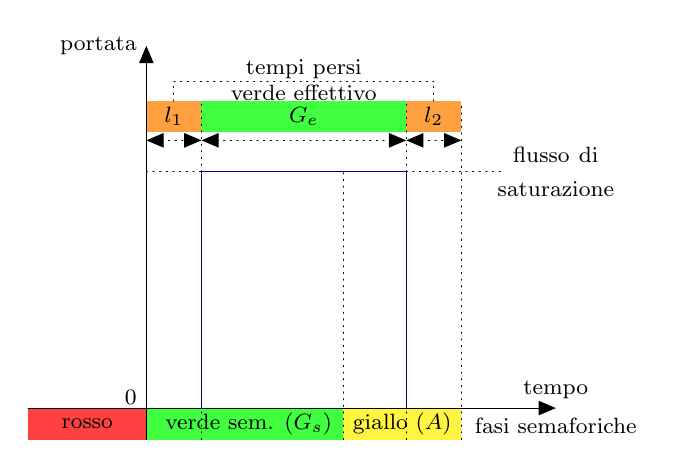
\begin{tikzpicture}[line cap=round,line join=round,>=triangle 45,x=0.1cm,y=0.1cm]

% barre sotto
\fill[red,opacity=.75] (-15,-4) rectangle (0,0);
\fill[green,opacity=.75] (0,-4) rectangle (25,0);
\fill[yellow,opacity=.75] (25,-4) rectangle (40,0);
%\fill[red] (40,-4) rectangle (52,0);

\draw[shift={(-7.5,-2)},color=black] node {\footnotesize rosso};
\draw[shift={(  13,-2)},color=black] node {\footnotesize verde sem. ($G_s$)};
\draw[shift={(32.5,-2)},color=black] node {\footnotesize giallo ($A$)};

%barre sopra
\fill[orange,opacity=.75] ( 0,35) rectangle ( 7,39);
\fill[green,opacity=.75]  ( 7,35) rectangle (33,39);
\fill[orange,opacity=.75]   ( 33,35) rectangle (40,39);

\draw[shift={( 3.5,37)},color=black] node {\footnotesize $l_1$};
\draw[shift={(  20,37)},color=black] node {\footnotesize $G_e$};
\draw[shift={(36.5,37)},color=black] node {\footnotesize $l_2$};

\draw[dotted] ( 3.5,39) -- ( 3.5,41.5);
\draw[dotted] (36.5,39) -- (36.5,41.5);
\draw[dotted] ( 3.5,41.5) -- (36.5,41.5);

\draw[shift={(  20,43)},color=black] node {\footnotesize tempi persi};
\draw[shift={(  20,40)},color=black] node {\footnotesize verde effettivo};

\draw[<->,color=black,dotted] ( 0,34) -- ( 7,34);
\draw[<->,color=black,dotted] ( 7,34) -- (33,34);
\draw[<->,color=black,dotted] (33,34) -- (40,34);

% l_1 stop
\draw[dotted] ( 7,-4) -- ( 7, 0);
\draw[dotted] ( 7,30) -- ( 7,39);
% giallo start0
\draw[dotted] (25,-4) -- (25,30);
% G_e stop
\draw[dotted] (33,-4) -- (33, 0);
\draw[dotted] (33,30) -- (33,39);
% l_2 stop
\draw[dotted] (40,-4) -- (40,39);

\draw[dotted] (0,30)-- ( 7,30);
\draw[dotted] (33,30)-- (45,30);
\node[text width=1.5cm,align=center] at (52, 30) {\footnotesize flusso di saturazione};

\draw[->,color=black] (-15,0) -- (52,0);
\draw[shift={(52,0)},color=black] node[above] {\footnotesize tempo};
\draw[shift={(52,0)},color=black] node[below] {\footnotesize fasi semaforiche};
\draw[->,color=black] (0,-4) -- (0,46);
\draw[shift={(0,46)},color=black] node[left] {\footnotesize portata};
\draw[color=black] (0pt,4pt) node[left] {\footnotesize $0$};

\draw[blue!50!black] (7,0)-- (7,30);
\draw[blue!50!black] (7,30)-- (33,30);
\draw[blue!50!black] (33,0)-- (33,30);

\color{red!50!black}
\draw plot[raw gnuplot, id=func0] function{set samples 100; set xrange [0:40]; plot 30*2.718281828**((-(x-20)**(6))/10000000)};

\clip(-15,-4) rectangle (60,46);

\end{tikzpicture}
\end{document} 
